\documentclass{article}

\usepackage{graphicx}
\usepackage{listings}
\lstset{basicstyle=\tiny}
\usepackage{float}

\usepackage{xepersian}
\settextfont{XB Zar}

\title{تمرین سری دوم درس سیستم‌های عامل پیشرفته}
\author{پارسا محمدیان -- 98102284}
\date{\today}

\begin{document}
\maketitle

\section{}
کد مربوط به این بخش در فایل 
\lr{1.c}
موجود است. اسکریپت اجرای آن نیز در فایل 
\lr{1.sh}
موجود است. 

اسکریپت همانطور که در تصاویر زیر نشان داده شده،‌ اجرا می‌شود. 
مقدار 
\lr{sleep}ای 
که قبل از دستور قرار داده شده است، برای این است که اسکریپت به صورت همزمان در هر دو ماشین 
اجرا شوند (دقت شود که ساعت سیستم با ساعت دو ماشین هماهنگ نیست ولی ساعت دو ماشین 
با هم هماهنگ است).
در ادامه این دستور 
\lr{sleep}
در فایل 
\lr{wait-untill.sh}
ذخیره و فراخوانی شده است.

\begin{figure}[H]
   \centering
   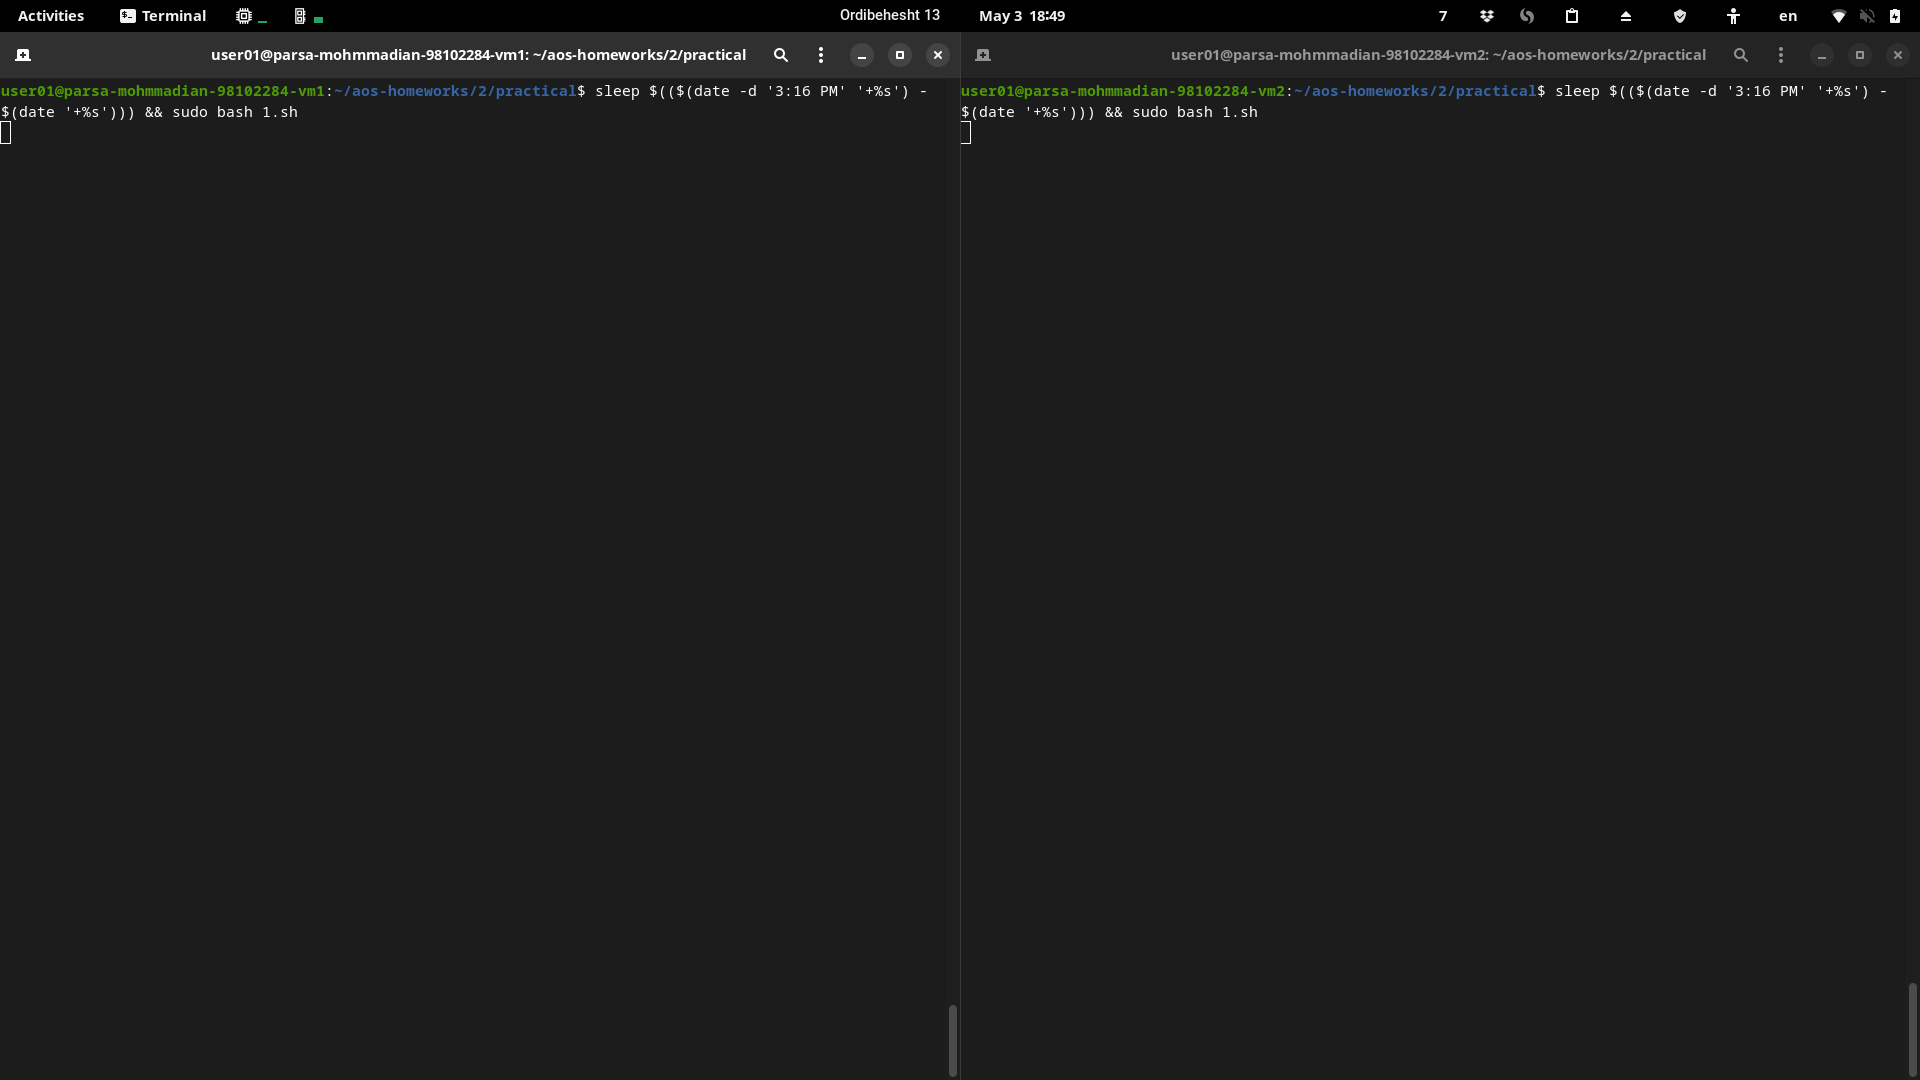
\includegraphics[width=\linewidth]{1-command.png}
\end{figure}
\begin{figure}[H]
   \centering
   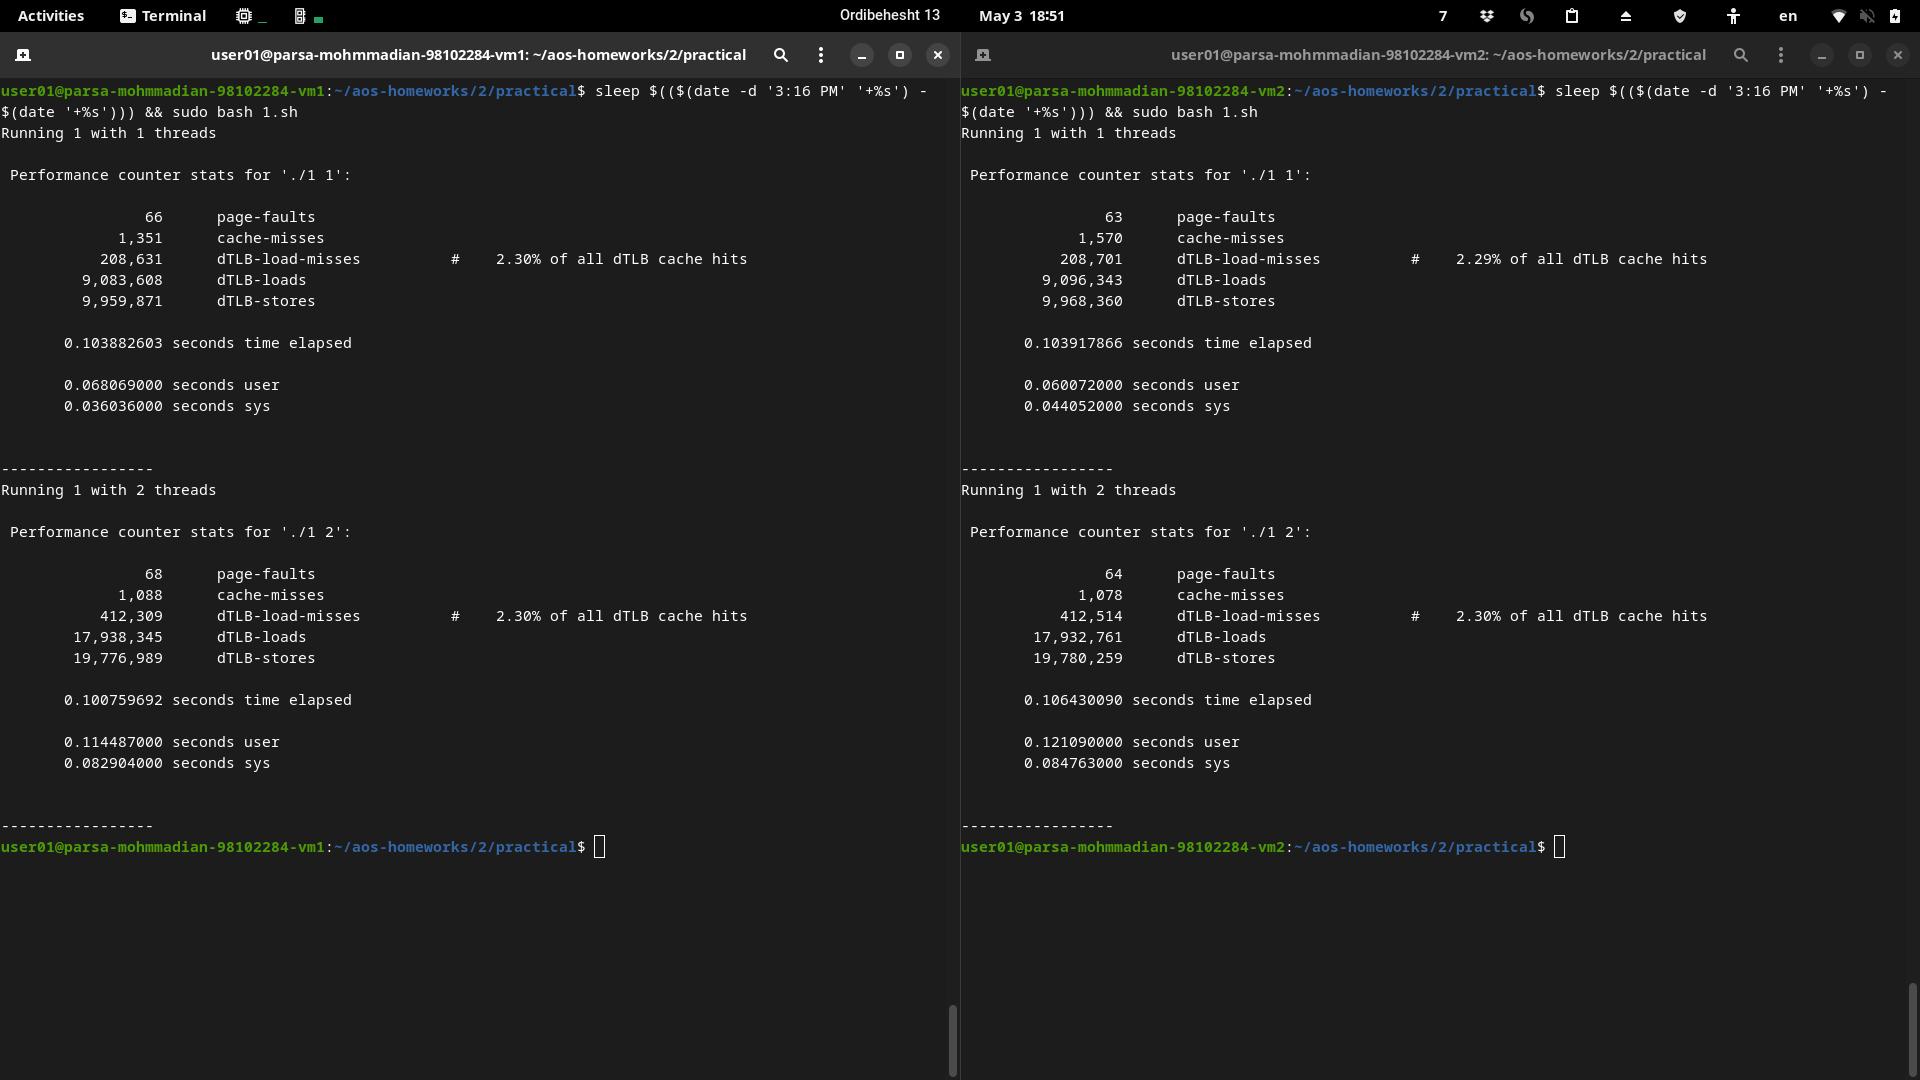
\includegraphics[width=\linewidth]{1-result.png}
\end{figure}

\subsection{}
آمار در ماشین مجازی اول به صورت زیر است. 
\begin{latin}
\begin{lstlisting}
Running 1 with 1 threads

 Performance counter stats for './1 1':

                66      page-faults                                                 
             1,351      cache-misses                                                
           208,631      dTLB-load-misses          #    2.30% of all dTLB cache hits 
         9,083,608      dTLB-loads                                                  
         9,959,871      dTLB-stores                                                 

       0.103882603 seconds time elapsed

       0.068069000 seconds user
       0.036036000 seconds sys


-----------------
Running 1 with 2 threads

 Performance counter stats for './1 2':

                68      page-faults                                                 
             1,088      cache-misses                                                
           412,309      dTLB-load-misses          #    2.30% of all dTLB cache hits 
        17,938,345      dTLB-loads                                                  
        19,776,989      dTLB-stores                                                 

       0.100759692 seconds time elapsed

       0.114487000 seconds user
       0.082904000 seconds sys
\end{lstlisting}
\end{latin}

آمار در ماشین مجازی دوم به صورت زیر است.
\begin{latin}
\begin{lstlisting}
Running 1 with 1 threads

 Performance counter stats for './1 1':

                63      page-faults                                                 
             1,570      cache-misses                                                
           208,701      dTLB-load-misses          #    2.29% of all dTLB cache hits 
         9,096,343      dTLB-loads                                                  
         9,968,360      dTLB-stores                                                 

       0.103917866 seconds time elapsed

       0.060072000 seconds user
       0.044052000 seconds sys


-----------------
Running 1 with 2 threads

 Performance counter stats for './1 2':

                64      page-faults                                                 
             1,078      cache-misses                                                
           412,514      dTLB-load-misses          #    2.30% of all dTLB cache hits 
        17,932,761      dTLB-loads                                                  
        19,780,259      dTLB-stores                                                 

       0.106430090 seconds time elapsed

       0.121090000 seconds user
       0.084763000 seconds sys
\end{lstlisting}
\end{latin}

\subsection{}
نتیجه اجرای این برنامه در تمرین اول نیز در ادامه قابل مشاهده است. 
\begin{latin}
\begin{lstlisting}
Running 1.3 with 1 threads

 Performance counter stats for './1.3':

                53      page-faults:u                                                         
             6,313      cache-misses:u                                                        
               167      dTLB-load-misses:u               #    0.52% of all dTLB cache accesses
            31,950      dTLB-loads:u                                                          
            11,341      dTLB-stores:u                                                         

       0.000851952 seconds time elapsed

       0.000867000 seconds user
       0.000000000 seconds sys


-----------------
Running 1.3 with 2 threads

 Performance counter stats for './1.3':

                51      page-faults:u                                                         
             6,226      cache-misses:u                                                        
               159      dTLB-load-misses:u               #    0.50% of all dTLB cache accesses
            31,950      dTLB-loads:u                                                          
            11,341      dTLB-stores:u                                                         

       0.000786024 seconds time elapsed

       0.000811000 seconds user
       0.000000000 seconds sys
\end{lstlisting}
\end{latin}
همانطور که مشاهده می‌کنیم،‌ این آمار در ماشین ۱ و ۲ تفاوت چندانی ندارند.
اما نسبت به نتایج آزمایش تمرین اول تغییرات قابل توجهی مشاهده می‌کنیم. 
در آزمایش جدید تعداد 
\lr{page-fault}ها 
تغییر چندانی نکرده است. تعداد 
\lr{cache-miss}ها
مقداری کاهش یافته است. تغییر اساسی در آمار مربوط به 
\lr{TLB}
است که به صورت محسوسی افزایش یافته‌اند.

\section{}
کد این برنامه در فایل 
\lr{2.c}
قرار دارد و اسکریپت اجرای آن در فایل 
\lr{2.sh}.
\subsection{}
ابتدا این برنامه را بر روی سیستم خودم اجرا کردم.
\begin{figure}[H]
   \centering
   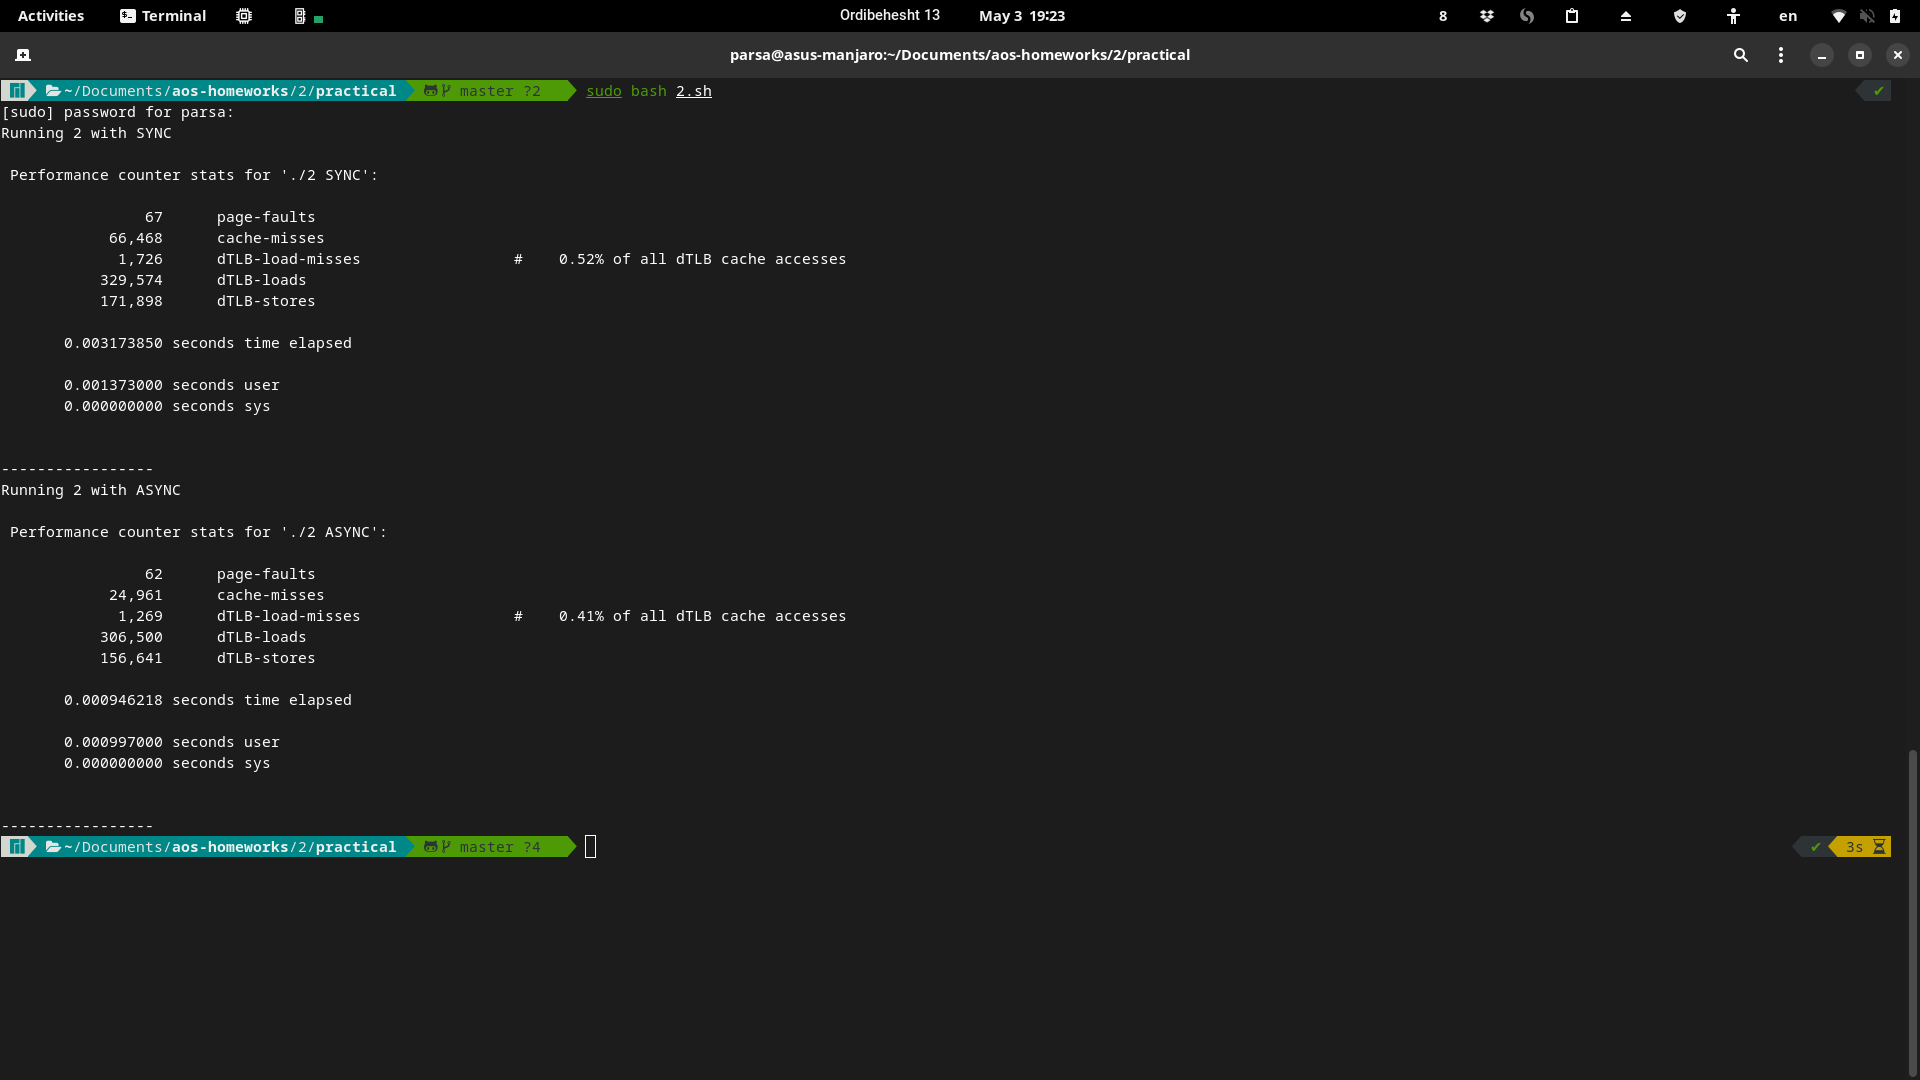
\includegraphics[width=\linewidth]{2-baremetal.png}
\end{figure}
نتایج به صورت زیر هستند.
\begin{latin}
\begin{lstlisting}
Running 2 with SYNC

 Performance counter stats for './2 SYNC':

                67      page-faults                                                           
            66,468      cache-misses                                                          
             1,726      dTLB-load-misses                 #    0.52% of all dTLB cache accesses
           329,574      dTLB-loads                                                            
           171,898      dTLB-stores                                                           

       0.003173850 seconds time elapsed

       0.001373000 seconds user
       0.000000000 seconds sys


-----------------
Running 2 with ASYNC

 Performance counter stats for './2 ASYNC':

                62      page-faults                                                           
            24,961      cache-misses                                                          
             1,269      dTLB-load-misses                 #    0.41% of all dTLB cache accesses
           306,500      dTLB-loads                                                            
           156,641      dTLB-stores                                                           

       0.000946218 seconds time elapsed

       0.000997000 seconds user
       0.000000000 seconds sys
\end{lstlisting}
\end{latin}

\subsection{}
\begin{figure}[H]
   \centering
   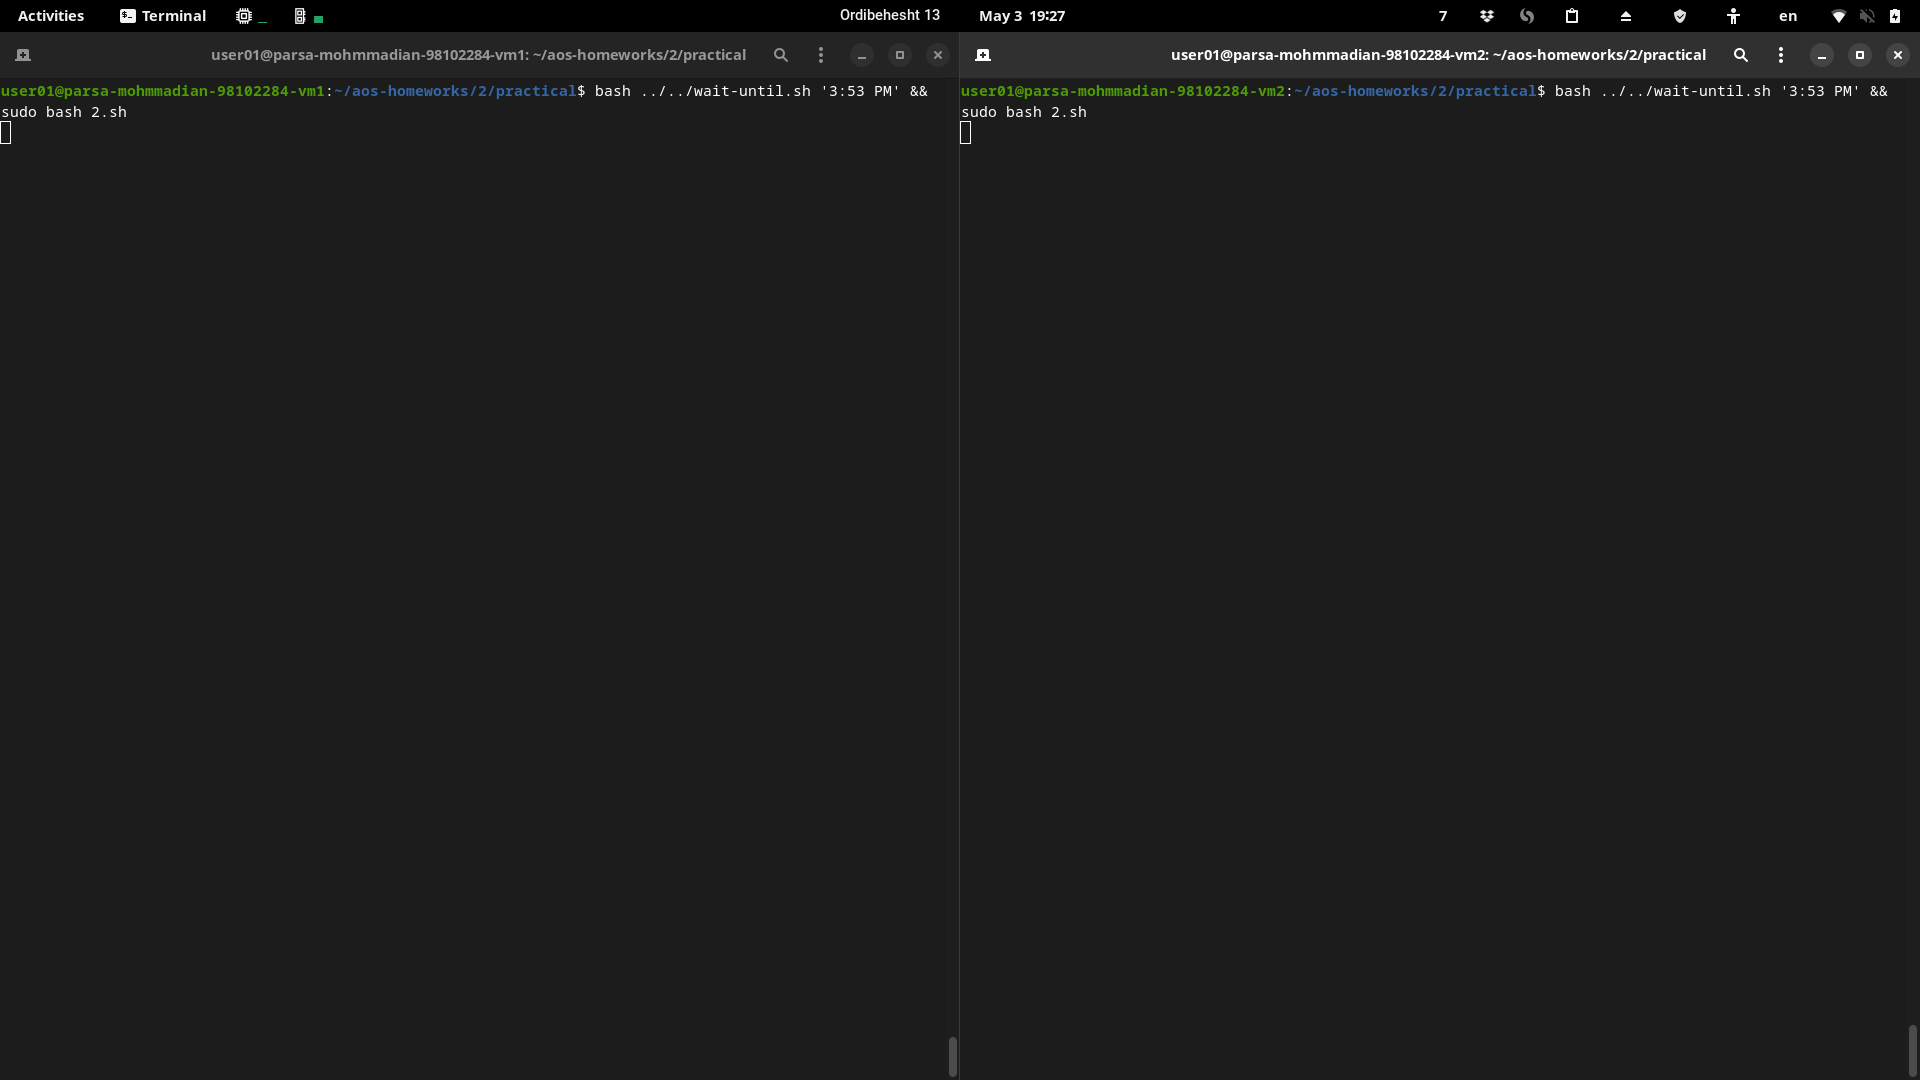
\includegraphics[width=\linewidth]{2-2-command.png}
\end{figure}
\begin{figure}[H]
   \centering
   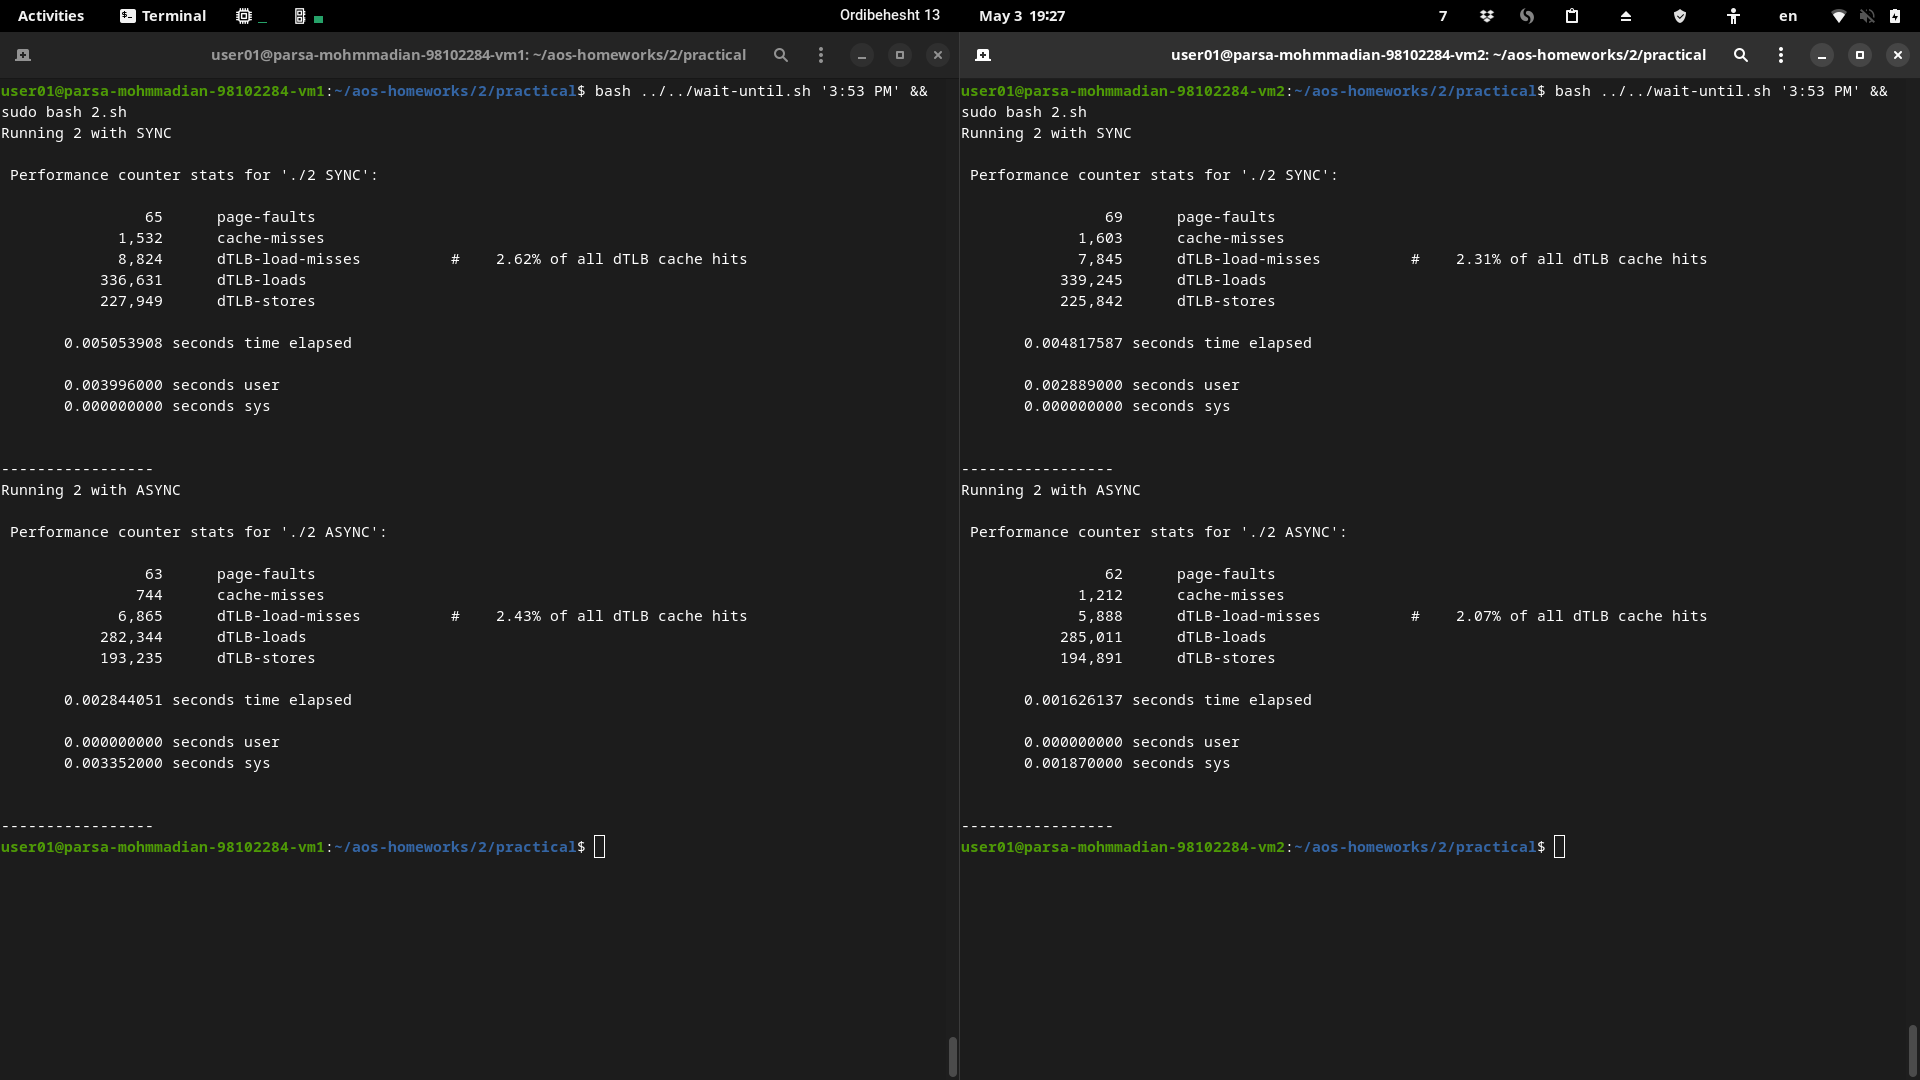
\includegraphics[width=\linewidth]{2-2-result.png}
\end{figure}

آمار در ماشین مجازی اول به صورت زیر است.
\begin{latin}
\begin{lstlisting}
Running 2 with SYNC

 Performance counter stats for './2 SYNC':

                65      page-faults                                                 
             1,532      cache-misses                                                
             8,824      dTLB-load-misses          #    2.62% of all dTLB cache hits 
           336,631      dTLB-loads                                                  
           227,949      dTLB-stores                                                 

       0.005053908 seconds time elapsed

       0.003996000 seconds user
       0.000000000 seconds sys


-----------------
Running 2 with ASYNC

 Performance counter stats for './2 ASYNC':

                63      page-faults                                                 
               744      cache-misses                                                
             6,865      dTLB-load-misses          #    2.43% of all dTLB cache hits 
           282,344      dTLB-loads                                                  
           193,235      dTLB-stores                                                 

       0.002844051 seconds time elapsed

       0.000000000 seconds user
       0.003352000 seconds sys
\end{lstlisting}
\end{latin}

آمار در ماشین مجازی دوم به صورت زیر است.
\begin{latin}
\begin{lstlisting}
   Running 2 with SYNC

   Performance counter stats for './2 SYNC':
  
                  69      page-faults                                                 
               1,603      cache-misses                                                
               7,845      dTLB-load-misses          #    2.31% of all dTLB cache hits 
             339,245      dTLB-loads                                                  
             225,842      dTLB-stores                                                 
  
         0.004817587 seconds time elapsed
  
         0.002889000 seconds user
         0.000000000 seconds sys
  
  
  -----------------
  Running 2 with ASYNC
  
   Performance counter stats for './2 ASYNC':
  
                  62      page-faults                                                 
               1,212      cache-misses                                                
               5,888      dTLB-load-misses          #    2.07% of all dTLB cache hits 
             285,011      dTLB-loads                                                  
             194,891      dTLB-stores                                                 
  
         0.001626137 seconds time elapsed
  
         0.000000000 seconds user
         0.001870000 seconds sys
\end{lstlisting}
\end{latin}

\subsection{}
تغییر بزرگی در این آمار‌ها وجود ندارد. صرفا 
\lr{cache miss}ها 
در اجرای ماشین مجازی کمتر هستند.

\subsection{}
همانطور که در خروجی‌های قسمت الف و ب مشاهده می‌کنیم،‌ برنامه یک بار 
برای 
\lr{MS\_ASYNC}
نیز اجرا شده. 

همانطور که مشاهده می‌شود، اکثر آمارها در اجرای 
\lr{MS\_ASYNC}
کاهش پیدا کرده‌اند. 

\section{}
این قسمت کدی به زبان 
\lr{C}
ندارد. اسکریپت مربوط به این قسمت در فایل 
\lr{3.sh}
می‌باشد. 
\subsection{}
ابتدا اسکریپت را روی سیستم خودم اجرا کردم.
\begin{figure}[H]
   \centering
   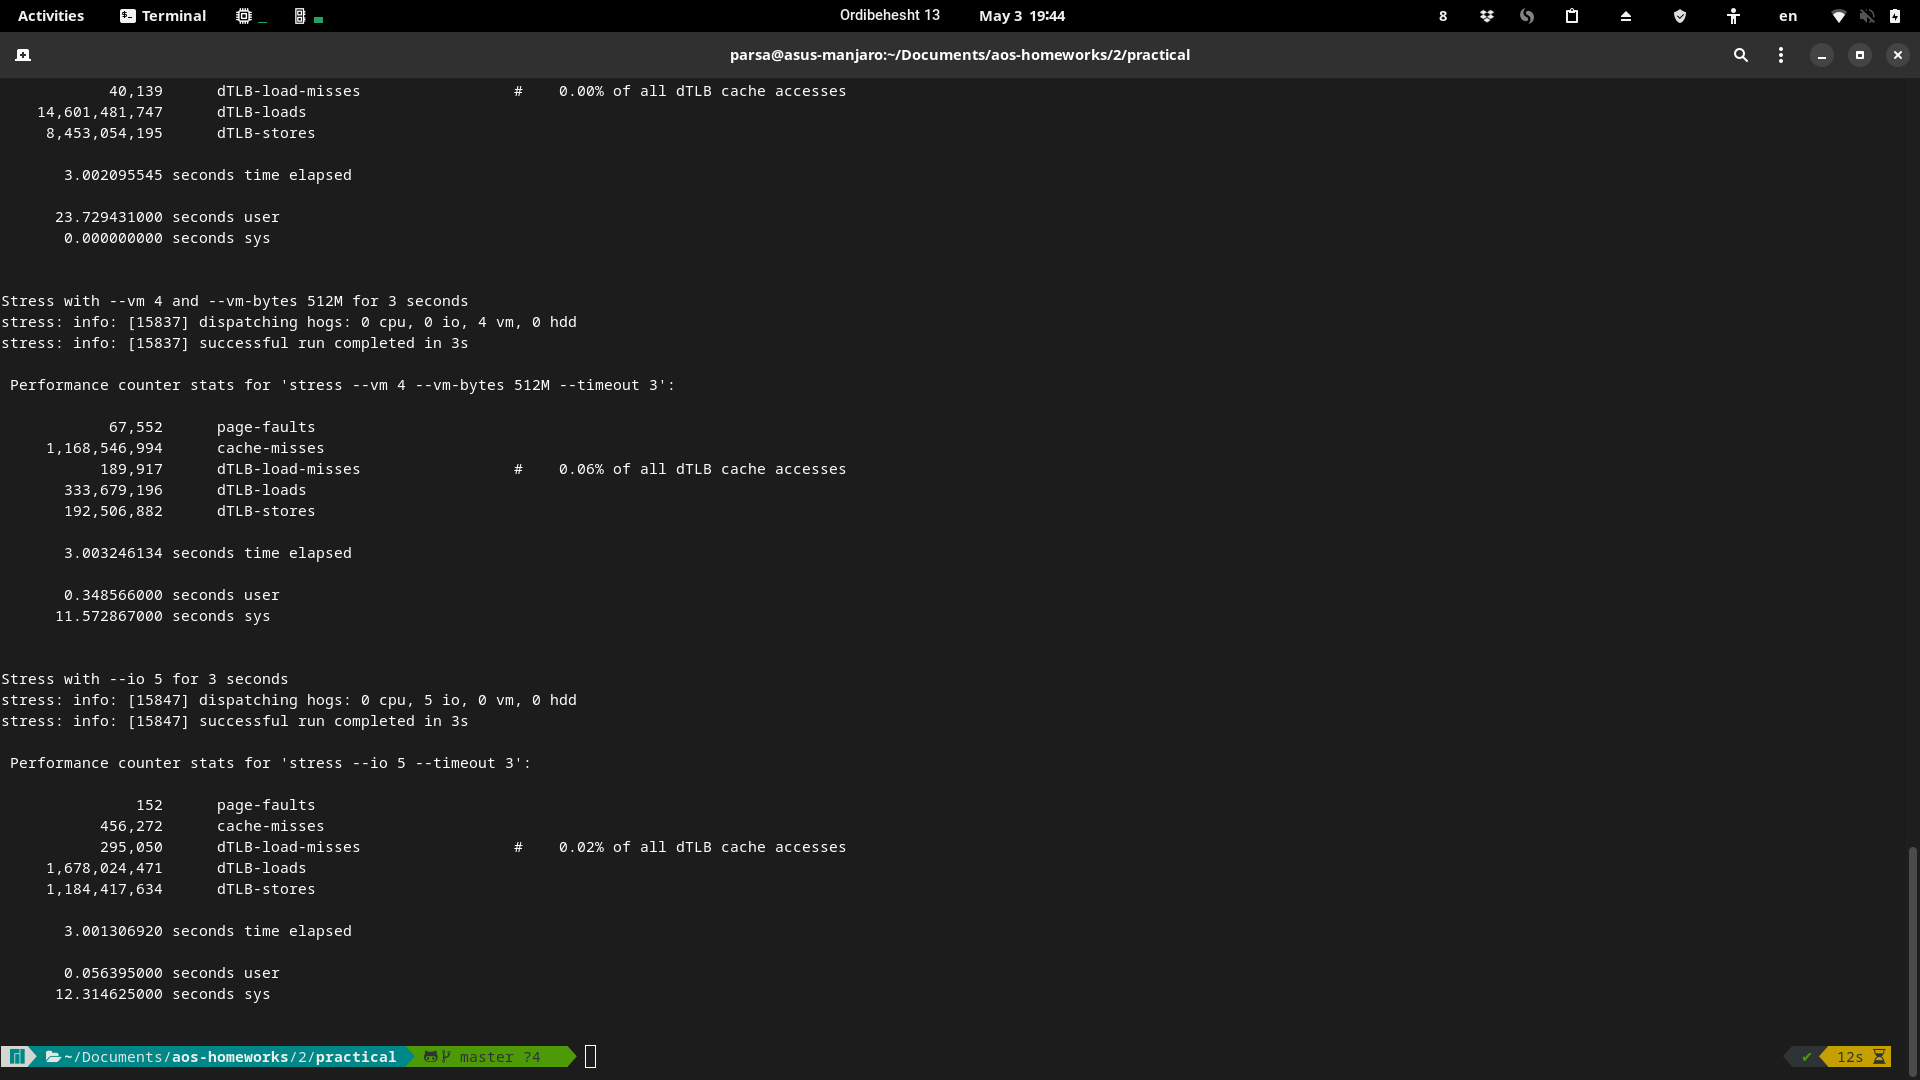
\includegraphics[width=\linewidth]{3-1.png}
\end{figure}

خروجی به صورت زیر است. 
\begin{latin}
\begin{lstlisting}
Running 3.sh
Stress with --cpu 10 for 30 seconds
stress: info: [18111] dispatching hogs: 10 cpu, 0 io, 0 vm, 0 hdd
7stress: info: [18111] successful run completed in 30s

 Performance counter stats for 'stress --cpu 10 --timeout 30':

               254      page-faults                                                           
         8,402,004      cache-misses                                                          
           516,139      dTLB-load-misses                 #    0.00% of all dTLB cache accesses
   141,800,586,533      dTLB-loads                                                            
    82,091,243,296      dTLB-stores                                                           

      30.002024177 seconds time elapsed

     233.838281000 seconds user
       0.195070000 seconds sys


Stress with --vm 4 and --vm-bytes 512M for 30 seconds
stress: info: [18241] dispatching hogs: 0 cpu, 0 io, 4 vm, 0 hdd
stress: info: [18241] successful run completed in 30s

 Performance counter stats for 'stress --vm 4 --vm-bytes 512M --timeout 30':

           601,603      page-faults                                                           
    10,564,193,883      cache-misses                                                          
         2,114,172      dTLB-load-misses                 #    0.07% of all dTLB cache accesses
     2,988,347,700      dTLB-loads                                                            
     1,723,228,183      dTLB-stores                                                           

      30.004263068 seconds time elapsed

       3.449375000 seconds user
     115.738466000 seconds sys


Stress with --io 5 for 30 seconds
stress: info: [18279] dispatching hogs: 0 cpu, 5 io, 0 vm, 0 hdd
stress: info: [18279] successful run completed in 30s

 Performance counter stats for 'stress --io 5 --timeout 30':

               141      page-faults                                                           
        35,274,133      cache-misses                                                          
         3,887,164      dTLB-load-misses                 #    0.03% of all dTLB cache accesses
    14,634,290,981      dTLB-loads                                                            
    10,328,414,193      dTLB-stores                                                           

      30.001919662 seconds time elapsed

       0.574676000 seconds user
     125.129620000 seconds sys
\end{lstlisting}
\end{latin}

\subsection{}
\begin{figure}[H]
   \centering
   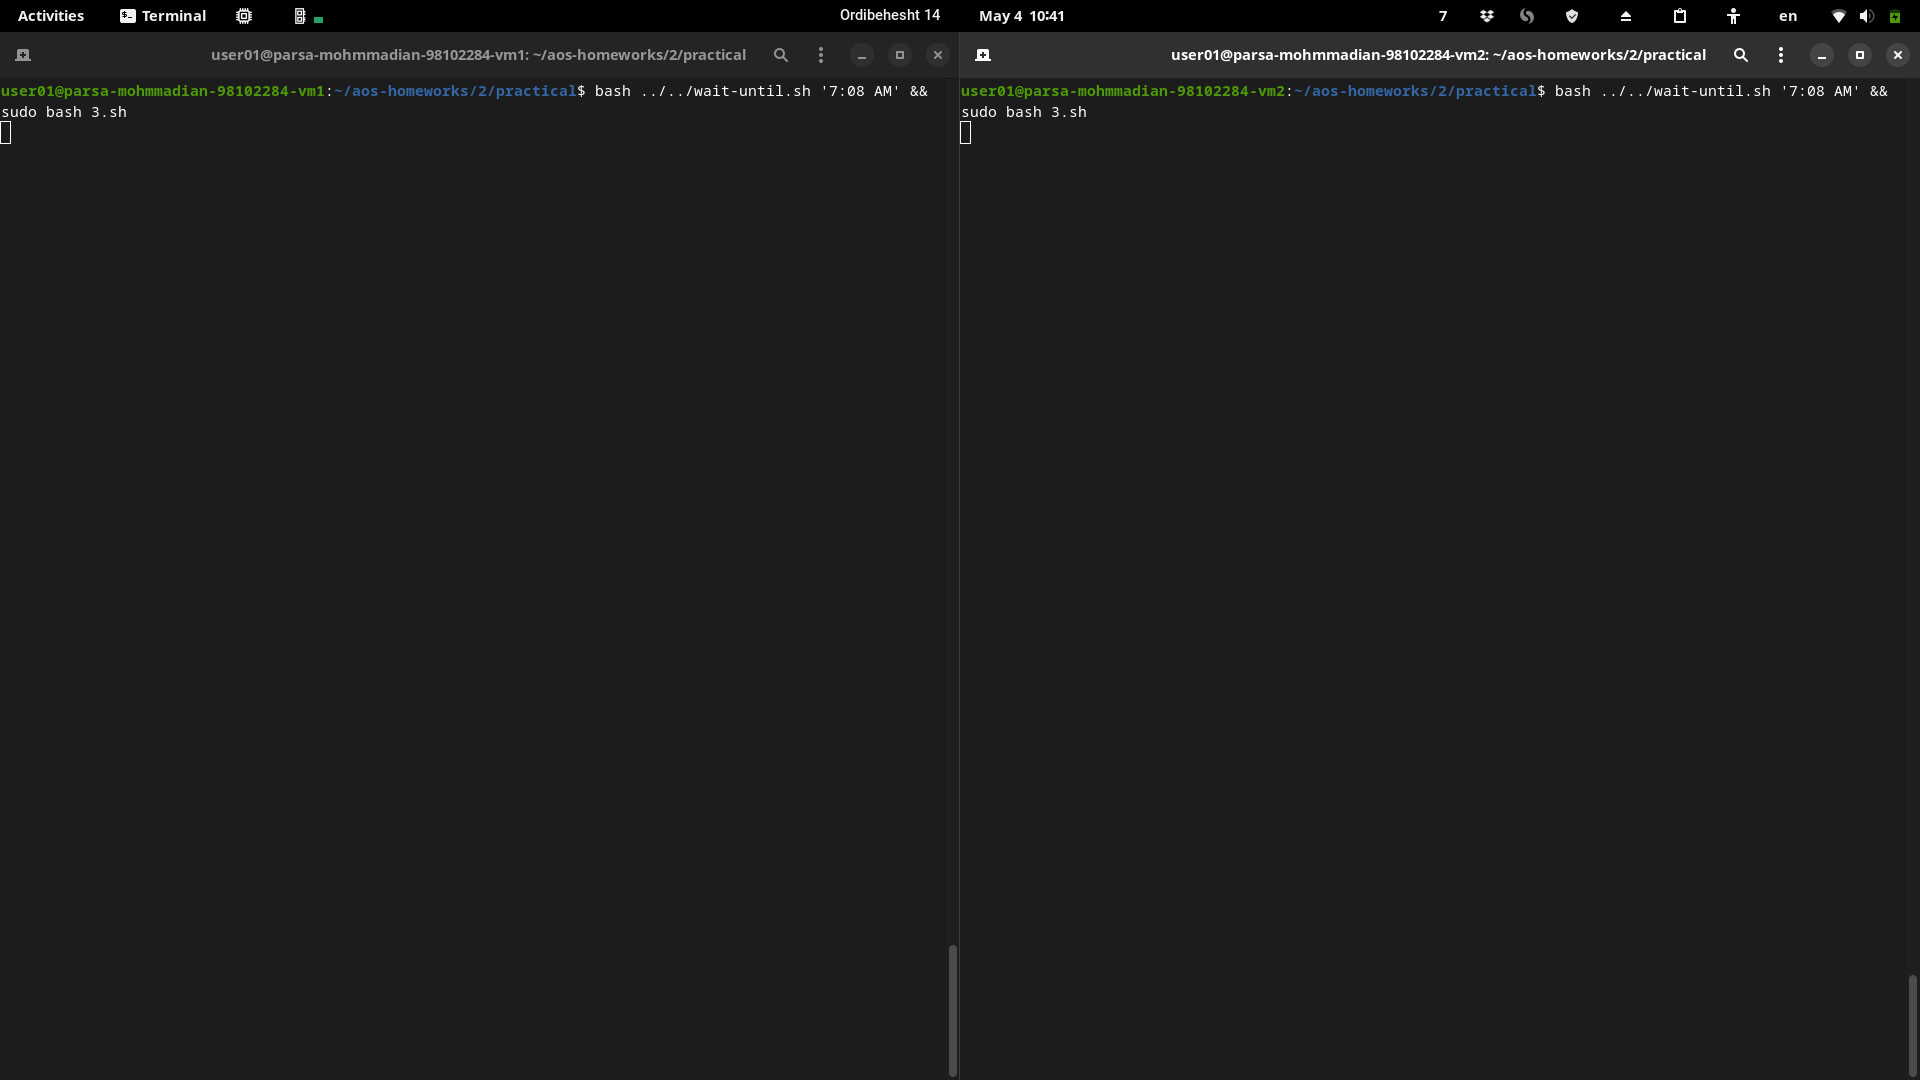
\includegraphics[width=\linewidth]{3-2-command.png}
\end{figure}
\begin{figure}[H]
   \centering
   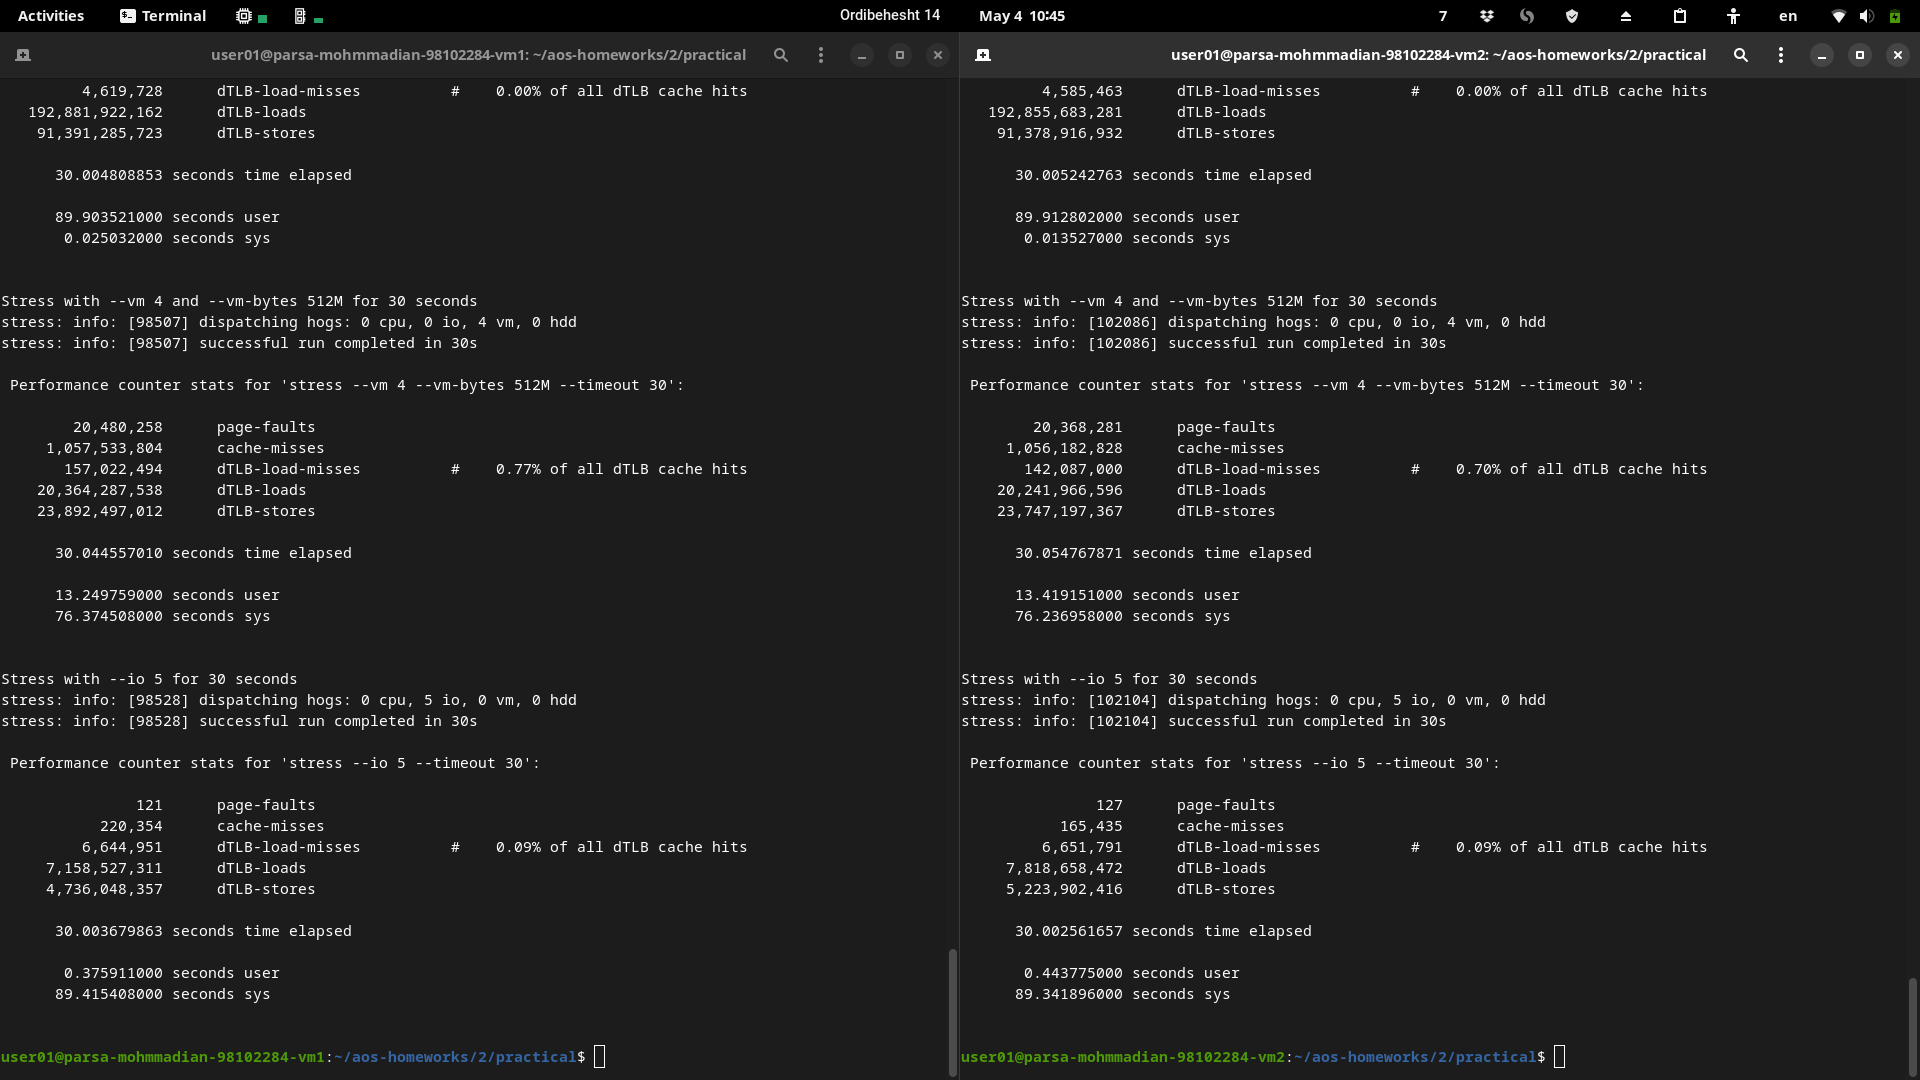
\includegraphics[width=\linewidth]{3-2-result.png}
\end{figure}

آمار در ماشین مجازی اول به صورت زیر است.
\begin{latin}
\begin{lstlisting}
Running 3.sh
Stress with --cpu 10 for 30 seconds
stress: info: [98481] dispatching hogs: 10 cpu, 0 io, 0 vm, 0 hdd
stress: info: [98481] successful run completed in 30s

 Performance counter stats for 'stress --cpu 10 --timeout 30':

               199      page-faults                                                 
           175,131      cache-misses                                                
         4,619,728      dTLB-load-misses          #    0.00% of all dTLB cache hits 
   192,881,922,162      dTLB-loads                                                  
    91,391,285,723      dTLB-stores                                                 

      30.004808853 seconds time elapsed

      89.903521000 seconds user
       0.025032000 seconds sys


Stress with --vm 4 and --vm-bytes 512M for 30 seconds
stress: info: [98507] dispatching hogs: 0 cpu, 0 io, 4 vm, 0 hdd
stress: info: [98507] successful run completed in 30s

 Performance counter stats for 'stress --vm 4 --vm-bytes 512M --timeout 30':

        20,480,258      page-faults                                                 
     1,057,533,804      cache-misses                                                
       157,022,494      dTLB-load-misses          #    0.77% of all dTLB cache hits 
    20,364,287,538      dTLB-loads                                                  
    23,892,497,012      dTLB-stores                                                 

      30.044557010 seconds time elapsed

      13.249759000 seconds user
      76.374508000 seconds sys


Stress with --io 5 for 30 seconds
stress: info: [98528] dispatching hogs: 0 cpu, 5 io, 0 vm, 0 hdd
stress: info: [98528] successful run completed in 30s

 Performance counter stats for 'stress --io 5 --timeout 30':

               121      page-faults                                                 
           220,354      cache-misses                                                
         6,644,951      dTLB-load-misses          #    0.09% of all dTLB cache hits 
     7,158,527,311      dTLB-loads                                                  
     4,736,048,357      dTLB-stores                                                 

      30.003679863 seconds time elapsed

       0.375911000 seconds user
      89.415408000 seconds sys
\end{lstlisting}
\end{latin}
آمار در ماشین مجازی دوم به صورت زیر است.
\begin{latin}
\begin{lstlisting}
Running 3.sh
Stress with --cpu 10 for 30 seconds
stress: info: [102060] dispatching hogs: 10 cpu, 0 io, 0 vm, 0 hdd
stress: info: [102060] successful run completed in 30s

 Performance counter stats for 'stress --cpu 10 --timeout 30':

               198      page-faults                                                 
           269,601      cache-misses                                                
         4,585,463      dTLB-load-misses          #    0.00% of all dTLB cache hits 
   192,855,683,281      dTLB-loads                                                  
    91,378,916,932      dTLB-stores                                                 

      30.005242763 seconds time elapsed

      89.912802000 seconds user
       0.013527000 seconds sys


Stress with --vm 4 and --vm-bytes 512M for 30 seconds
stress: info: [102086] dispatching hogs: 0 cpu, 0 io, 4 vm, 0 hdd
stress: info: [102086] successful run completed in 30s

 Performance counter stats for 'stress --vm 4 --vm-bytes 512M --timeout 30':

        20,368,281      page-faults                                                 
     1,056,182,828      cache-misses                                                
       142,087,000      dTLB-load-misses          #    0.70% of all dTLB cache hits 
    20,241,966,596      dTLB-loads                                                  
    23,747,197,367      dTLB-stores                                                 

      30.054767871 seconds time elapsed

      13.419151000 seconds user
      76.236958000 seconds sys


Stress with --io 5 for 30 seconds
stress: info: [102104] dispatching hogs: 0 cpu, 5 io, 0 vm, 0 hdd
stress: info: [102104] successful run completed in 30s

 Performance counter stats for 'stress --io 5 --timeout 30':

               127      page-faults                                                 
           165,435      cache-misses                                                
         6,651,791      dTLB-load-misses          #    0.09% of all dTLB cache hits 
     7,818,658,472      dTLB-loads                                                  
     5,223,902,416      dTLB-stores                                                 

      30.002561657 seconds time elapsed

       0.443775000 seconds user
      89.341896000 seconds sys
\end{lstlisting}
\end{latin}

\subsection{}
برای هر کدام از تست‌ جداگانه بررسی می‌کنیم. از آنجایی که آمار 
دو ماشین مجازی نسبت به هم تفاوت زیادی ندارد، دو ماشین مجازی 
را با حالت 
\lr{baremetal}
مقایسه می‌کنیم. 

\begin{enumerate}
  \item در این تست 
  \lr{cache misses}
  در حالت 
  \lr{baremetal}
  بیشتر از حالت ماشین مجازی است. اما در مقابل 
  \lr{TLB load misses}
  کمتر است. و بقیه آمارها نیز تفاوت زیادی ندارند.
  \item در این تست همه آمارها به غیر از 
  \lr{cache misses}
  در حالت ماشین مجازی بیشتر شده‌اند.
  \item در تست آخر که مربوط به 
  \lr{IO}
  است، آمارها در حالت 
  \lr{baremetal}
  بیشتر شده‌اند.
\end{enumerate}

\end{document}